\documentclass[12pt, twoside]{article}
\usepackage[letterpaper, margin=1in, headsep=0.5in]{geometry}
\usepackage[english]{babel}
\usepackage[utf8]{inputenc}
\usepackage{amsmath}
\usepackage{amsfonts}
\usepackage{amssymb}
\usepackage{tikz}
\usetikzlibrary{quotes, angles}
\usepackage{graphicx}
\usepackage{enumitem}
\usepackage{multicol}

\newif\ifmeta
\metatrue %print standards and topics tags

\title{Regents Geometry}
\author{Chris Huson}
\date{September 2020}

\usepackage{fancyhdr}
\pagestyle{fancy}
\fancyhf{}
\renewcommand{\headrulewidth}{0pt} % disable the underline of the header
\raggedbottom


\fancyhead[LE]{\thepage}
\fancyhead[RO]{\thepage \\ Name: \hspace{4cm} \,\\}
\fancyhead[LO]{BECA / Dr. Huson / Geometry 10-Trig+similarity+analytics\\* pset ID: 170}

\begin{document}

\subsubsection*{10-4bDN-Analytics-review}
\begin{enumerate}
\item Write down the slope parallel or perpendicular to the given slope. \vspace{0.5cm}
  \begin{enumerate}
    \begin{multicols}{2}
      \item   $m= -1.25 \hspace{1cm} m_{\parallel} = $ \vspace{1cm}
      \item   $m= -\frac{3}{7} \hspace{1cm} m_{\parallel} = $
      \item   $m= -\frac{3}{2} \hspace{1cm} m_{\perp} = $ \vspace{1cm}
      \item   $m= 0.8 \hspace{1cm} m_{\perp} = $
    \end{multicols}
  \end{enumerate}\vspace{0.15cm}

\item Rewrite each linear equation in slope-intercept form.
  \begin{enumerate}
    \begin{multicols}{2}
    \item   $2x-y=-6$
    \item   $5x-2y=6$
    \end{multicols}
  \end{enumerate}  \vspace{3cm}

  In the following problems, use the point-slope formula: $y-y_1=m (x-x_1)$
\item What is the equation of a line through $(1,7)$ parallel to the line $y=-\frac{1}{3}x+7$?  \vspace{3cm}
\item What is the equation of a line through $(2,-2)$ perpendicular to the line $y=\frac{3}{5}x+1$?  \vspace{3cm}
\item What is the equation of a line through $(3,-1)$ perpendicular to the line $4x+2y=6$?  \vspace{3cm}

\newpage  
\item What is an equation of the perpendicular bisector of $\overline{AB}$ with $A(2,1)$ and $B(-4,-5)$? 
  \begin{flushright}
    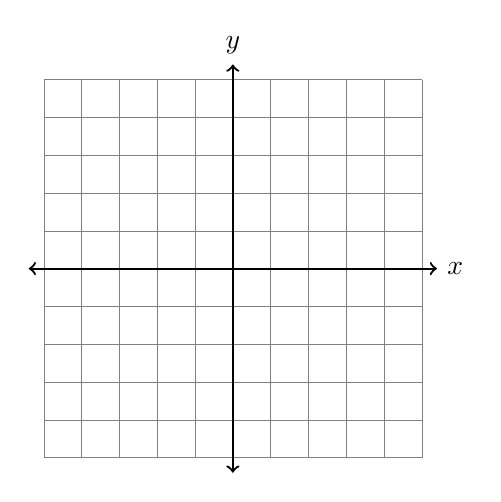
\begin{tikzpicture}[scale=.48]
    \draw [help lines] (-5,-5) grid (5,5);
    \draw [thick, <->] (-5.4,0) -- (5.4,0) node [right] {$x$};
    \draw [thick, <->] (0,-5.4)--(0,5.4) node [above] {$y$};   
  \end{tikzpicture}
\end{flushright}

\item Describe a rigid motion that maps $\triangle TIC$ onto $\triangle TOK$. 
  \begin{flushright}
      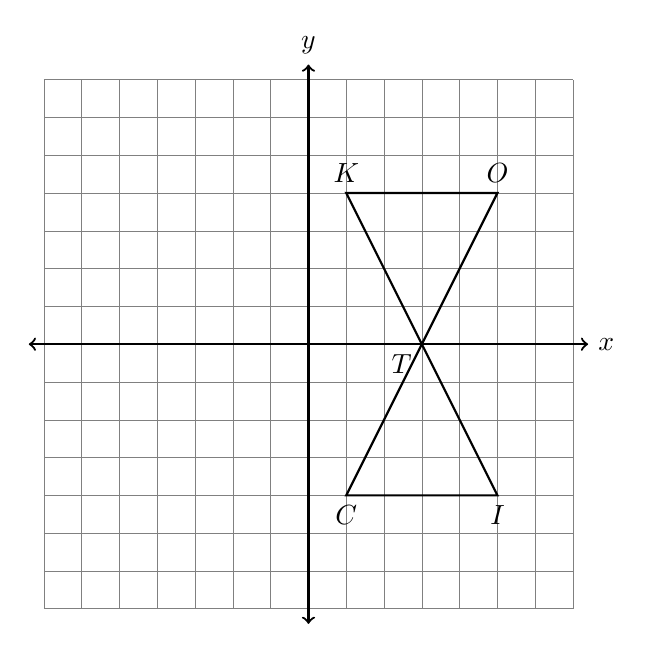
\begin{tikzpicture}[scale=.48]
      \draw [help lines] (-7,-7) grid (7,7);
      \draw [thick, <->] (-7.4,0) -- (7.4,0) node [right] {$x$};
      \draw [thick, <->] (0,-7.4)--(0,7.4) node [above] {$y$};  
      \draw [thick]
        (1,4) node[above] {$K$}--
        (5,4) node[above] {$O$}--
        (3,0) --cycle;
      \draw [thick]
      (1,-4) node[below] {$C$}--
      (5,-4) node[below] {$I$}--
      (3,0) node[below left] {$T$}--cycle;
    \end{tikzpicture}
  \end{flushright}

\item Mark the missing labels for a rotation of $180^\circ$ counterclockwise around $C$ of $\triangle ABC$ onto $\triangle A'B'C'$, and for a reflection across $l$ of $\triangle DEF$ onto $\triangle D'E'F'$. \vspace{1cm}
\begin{center}
      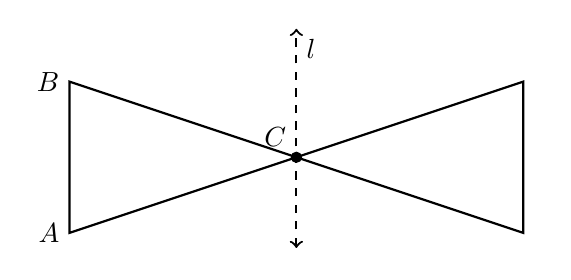
\begin{tikzpicture}[scale=.48]
      %\draw [help lines] (-8,-8) grid (7,5);
      %\draw [thick, <->] (-8.4,0) -- (7.4,0) node [right] {$x$};
      \draw [thick, <->, dashed] (0,-5.4)--(0,0.4) node [below right] {$l$};  
      \draw [thick]
        (-6,-1) node[left] {$B$}--
        (-6,-5) node[left] {$A$}--
        (0,-3) node[above left] {$C$}--cycle;
      \fill (0,-3) circle[radius=0.15cm];
      \draw [thick]
      (6,-1) node[right] {}--
      (6,-5) node[above right] {}--
      (0,-3) node[below right] {}--cycle;
    \end{tikzpicture} \hspace{1cm}
    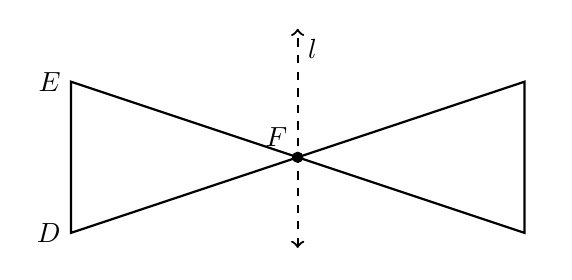
\begin{tikzpicture}[scale=.48]
      %\draw [help lines] (-8,-8) grid (7,5);
      %\draw [thick, <->] (-8.4,0) -- (7.4,0) node [right] {$x$};
      \draw [thick, <->, dashed] (0,-5.4)--(0,0.4) node [below right] {$l$};  
      \draw [thick]
        (-6,-1) node[left] {$E$}--
        (-6,-5) node[left] {$D$}--
        (0,-3) node[above left] {$F$}--cycle;
      \fill (0,-3) circle[radius=0.15cm];
      \draw [thick]
      (6,-1) node[right] {}--
      (6,-5) node[above right] {}--
      (0,-3) node[below right] {}--cycle;
    \end{tikzpicture}
  \end{center} \vspace{1cm}

\newpage
\item Find the image of $G(2,-5)$ after a rotation of $90^\circ$ counterclockwise around the origin.
  \begin{flushright}
    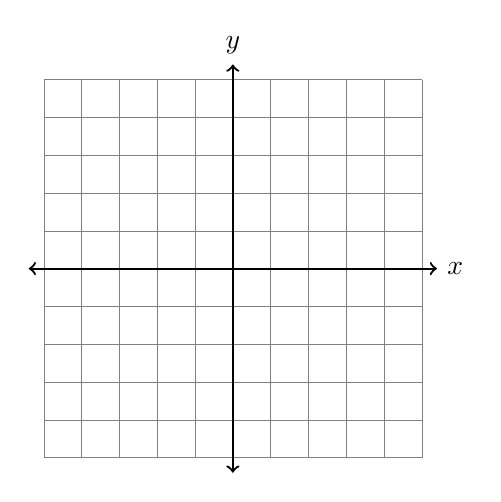
\begin{tikzpicture}[scale=.48]
    \draw [help lines] (-5,-5) grid (5,5);
    \draw [thick, <->] (-5.4,0) -- (5.4,0) node [right] {$x$};
    \draw [thick, <->] (0,-5.4)--(0,5.4) node [above] {$y$};   
  \end{tikzpicture}
\end{flushright}

\item Describe a rigid motion that maps $\triangle TIC$ onto $\triangle TOK$. 
  \begin{flushright}
      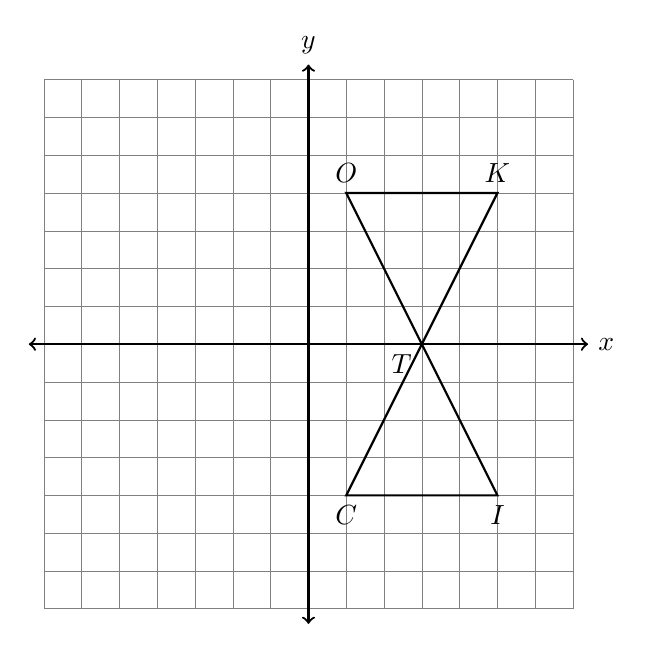
\begin{tikzpicture}[scale=.48]
      \draw [help lines] (-7,-7) grid (7,7);
      \draw [thick, <->] (-7.4,0) -- (7.4,0) node [right] {$x$};
      \draw [thick, <->] (0,-7.4)--(0,7.4) node [above] {$y$};  
      \draw [thick]
        (1,4) node[above] {$O$}--
        (5,4) node[above] {$K$}--
        (3,0) --cycle;
      \draw [thick]
      (1,-4) node[below] {$C$}--
      (5,-4) node[below] {$I$}--
      (3,0) node[below left] {$T$}--cycle;
    \end{tikzpicture}
  \end{flushright}

\item Find the coordinates of the image of $G(-2,-3)$ after a reflection across the $x$-axis.
  \begin{flushright}
    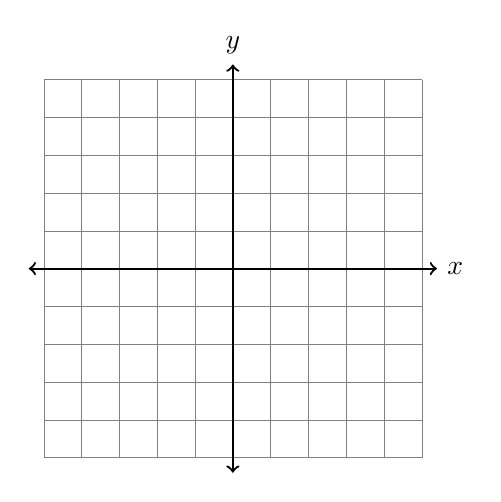
\begin{tikzpicture}[scale=.48]
    \draw [help lines] (-5,-5) grid (5,5);
    \draw [thick, <->] (-5.4,0) -- (5.4,0) node [right] {$x$};
    \draw [thick, <->] (0,-5.4)--(0,5.4) node [above] {$y$};   
  \end{tikzpicture}
\end{flushright}

\end{enumerate}
\end{document}